% Created 2019-10-04 Fri 00:59
\documentclass[11pt]{article}
\usepackage[utf8]{inputenc}
\usepackage[T1]{fontenc}
\usepackage{fixltx2e}
\usepackage{graphicx}
\usepackage{grffile}
\usepackage{longtable}
\usepackage{wrapfig}
\usepackage{rotating}
\usepackage[normalem]{ulem}
\usepackage{amsmath}
\usepackage{textcomp}
\usepackage{amssymb}
\usepackage{capt-of}
\usepackage{hyperref}
\author{Fabio Favero Henkes}
\date{\today}
\title{}
\hypersetup{
 pdfauthor={Fabio Favero Henkes},
 pdftitle={},
 pdfkeywords={},
 pdfsubject={},
 pdfcreator={Emacs 24.5.1 (Org mode 8.3.4)},
 pdflang={English}}
\begin{document}

\tableofcontents

\section{Objetivo}
\label{sec:orgheadline1}

O objetivo do jogo é tornar-se o mais venerável de todo o reino do rei Daniel.

\section{Mapa}
\label{sec:orgheadline2}

Dividido em 6 partes: mar (pequenas ilhas), grandes ilhas, floresta, deserto, terra desolada e montanhas. As seis localidades iniciais são circuladas em rosa.

Tiles de região: para cada região há um conjunto de tiles que servem para avançar nas épocas do jogo que é dividido em 5 (épocas). Ao atingir a 5a época o jogo termina e a pontuação final ocorre.

Gráficos: existem dois gráficos no tabuleiro representando o avanço das épocas (tiles que precisam ser removidos em cada uma para avançar para a próxima) e o gráfico de evolução de área.
(para cada tipo de localidade qual sua escala de evolução, ex: cidade -> feudum).

Barris de vinho: na cor do jogador onde é possível armazenar enxofre para a fermentação de vinho.

Guildas: 6 guildas circundando o tabuleiro.

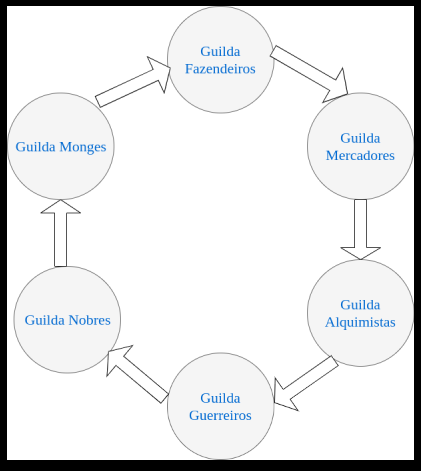
\includegraphics[width=.9\linewidth]{./img/guilds.png}

(As guildas relacionam-se umas com as outras conforme acima)

\section{Sacola de recursos (mochila)}
\label{sec:orgheadline3}

Todos os recursos aleatórios do jogo são armazenados.

\section{Área do jogador (tableau)}
\label{sec:orgheadline4}

Cada jogador recebe o mesmo set de componentes com uma pequena diferença de recursos.

\begin{itemize}
\item 11 cartas de ação na cor do jogador
\item 3 peões de 6 lados na cor do jogador representando diferenetes personagens relacionados às guildas
\item 7 marcadores de influência na cor do jogador (mais podem ser conseguidos durante a partida)
\item 4 discos na cor do jogador (dois para uso de guardiões no jogo avançado, que possuem um desenho de ponto de vitória)
\item 7 xelins (dinheiro)
\item 7 recursos de comida
\item 3 recursos diferentes quaisquer a escolha do jogador
\item 1 token de sacola na cor do jogador
\end{itemize}

\section{O jogo}
\label{sec:orgheadline5}

O jogo é dividido em 5 épocas nas quais um número indeterminado de rounds pode ser jogado, as épocas avançam conforme os tiles de região são descobertos e ao atingir a 5 época o jogo acaba e são contados os pontos de vitória.


Um round consiste em 5 passos ou fases:

\begin{itemize}
\item 1) Selecionar 4 das 11 cartas disponíveis e executar suas ações em ordem de turno de jogadores;
\item 2) Alimentar os peões no tabuleiro (comida ou vinho)
\item 3) Rolar o dado de progresso, isso é feito pelo jogador inicial e indica qual tile de região deverá ser removido do jogo.
\item 4) Caso atingida a mudança de época o marcador de época é avançado e a pontuação da época executada.
\end{itemize}
O tabuleiro nesse caso é repopulado conforme descrito na mudança época no manual do jogo. Caso a 5 época tenha sido atingida, após a pontuação de época segue-se para a pontuação de final de jogo.
\begin{itemize}
\item 5) Passar o marcador de primeiro jogador em sentido horário e o dado de progresso, caso a 5 época ainda não tenha sido atingida.
\end{itemize}

\section{Ações do jogador}
\label{sec:orgheadline7}

Escolha 4 dentre as 11 cartas disponíveis para jogar no round.

Após a escolha das cartas o jogador inicial randomicamente escolhido começa.

Alguns símbolos podem aparecer nas cartas

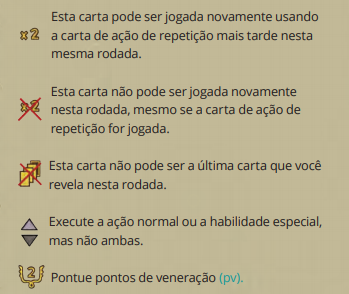
\includegraphics[width=.9\linewidth]{./img/symbol.png}

\begin{itemize}
\item Ação normal: qualquer jogador pode executar a ação normal descrita na seção superior da carta.
\item Ação extra: o jogador pode gastar um recurso de salitre para adicionar uma quinta carta a sua mão nesta rodada.
\item Ação sequencial: o jogador pode gastar um recurso de enxofre para jogar duas cartas em um único turno.
\end{itemize}

Caso o jogador assim escolha, poderá executar apenas uma das ações (extra ou sequencial) por rodada, colocando o recurso correspondente em seu token de sacola na sua área de jogador
para demonstrar aos demais jogadores sua opção.
Após a execução da ação o recurso deve ser descartado no sacola de recursos.

\begin{itemize}
\item Habilidade especial: A posse de determinado recurso, ou de um peão específico permite a utlização da habilidade especial.
\end{itemize}

O jogador DEVE jogar ao menos uma carta por turno mas PODE DESISTIR da ação.

\subsection{As 11 cartas de ação}
\label{sec:orgheadline6}


\textbf{1) Ação migrar:} o jogador pode migrar um de seus peões para dentro ou fora do tabuleiro de jogo. Caso opte por migrar um peão para dentro do tabuleiro, deve pagar uma comida.
O peão deve ser colocado ao lado de outro peão do jogador ou um de seus marcadores de influência, caso não possua nenhum peão no tabuleiro coloque o mesmo próximo a uma das localidades
iniciais. Então escolha a face do peão que representa o personagem desejado (fazendeiro, mercador, alquimista, guerreiro, nobre ou monge).

\textbf{1.1) Habilidade especial "Parente distante":} Caso já possua um peão no tabuleiro do tipo alquimista, o jogador pode escolher colocar o peão em alguma das localidades iniciais do jogo,
sem a necessidade de estar junto a outro de seus peões ou marcadores de influência.

Obs: Ao colocar um peão de respectivo personagem no tabuleiro este irá fornecer ao jogador status na respectiva guilda. Verifique sua influência na guilda neste momento. Cada guilda possui critérios
específicos para fornecer mais status aos jogadores (peões, feudums, postos avançados, etc). O jogador com mais influẽncia na guilda recebe o título de mestre e coloca seu marcador de influência
no espaço de 5vps a ser ganho na virada de época, o segundo jogador recebe o título de oficial e coloca seu marcador no espaço de 3vps.

\textbf{2) Ação de repetir:} esta ação permite que o jogador repita a ação de qualquer carta jogada durante a rodada, desde que a mesma possua o símbolo de repetição no canto superior direito.

\textbf{2.1) Habilidade especial "Deja vu":} caso o jogador devolva um salitre para a sacola de recursos é possível executar a carta que não possuir o símbolo de repetição uma segunda
vez na rodada. Cartas com os símbolos 2x riscados (conquista e defesa) nunca podem ser repetidas.

\textbf{3) Ação mover:} sua permissão de movimento total é igual ao número de peões que possui no tabuleiro, estes movimentos podem ser divididos entre todos os peões. O jogador pode se deslocar
por estradas ou rotas de embarcações especiais.

     Furtando recursos: ao final de sua ação de movimento se um de seus peões estiver ao lado de de localidades com recursos vc pode furtar 1 deles a sua escolha, apenas um de seus peões pode
fazê-lo mesmo que hajam mais peões junto a recursos. Não é possível furtar de um local que vc mesmo domine ou que vc possua um servo.
Caso escolha um enxofre o mesmo pode ir para seus suprimentos (tableu) ou para seu barril de vinho.

     Embarcações: se o jogador tiver uma embarcação poderá se deslocar pelas rotas especiais, sendo rota de submarino (bolhas), rota de navio (ondas) ou rota de voo (passáros). O jogador
pode abandonar a embarcação e continuar o movimento pela estrada, mas a mesma poderá ser usada por qualquer um daqui pra frente. Embarcações podem ser adquiridas na guilda do alquimista.

Balsas: Caso o alquimista não possua mais embarcações para a venda, as balsas podem ser usadas mediante o pagamento de 2 xelins.

     Viagem épica: Caso vc jogue a ação mover por duas vezes com sucesso na rodada (vide carta de repetir) avance na trilha de viagem épica ao encontrar um espaço com ícone de carta
compre 2 cartas de escritura real e fique com 1 devolvendo a outra para o fundo do baralho. A viagem é pontuada ao final do jogo sendo que o primeiro jogador na trilha pontua o maior
valor da seção onde se encontra, caso empate ambos pontuam o maior valor. No final da trilha há o monastério, qualquer marcador que o atingir marcará 17pvs.

\textbf{3.1) Habilidade especial "boa sorte":} Caso o jogador possua um peão monge no tabuleiro este pode adicionar +1 ao seu movimento. Escolha um de seus peões monge para a habilidade.
Qualquer peão independente do personagem pode ser movido.

\textbf{4) Ação de Influência:} o jogador pode adicionar um marcador de influência para cada local que houver um de seus peões. Cada localidade pode conter no máximo tres marcadores
pertencentes a dois jogadores.

Soberanos, súditos e servos: O primeiro jogador a adicionar um marcador de influência no local torna-se o soberano, o segundo e diferente jogador coloca o marcador ao lado sendo
o servo garantindo o direito de guardar o terreno. No futuro qualquer um dos dois jogadores pode adicionar um marcador de influência final, caso já seja vc o soberano adicione este
marcador ao lado tornando-se o súdito, caso vc seja o servo, tome o lugar do soberano rebaixando o mesmo a servo e tornando seu outro marcador súdito.

Obs: algumas localidades podem aumentar status em algumas guildas, verifique os status neste momento.

\textbf{4.1) Habilidade especial "dinheiro é influência":} se o jogador tiver o peão de comerciante em um local governado por um único marcador de oponente (ou seja não há súdito), pague 1 xelim
para mover o soberano da região para a posição de servo e coloque um de seus marcadores de influência como soberano na localidade. Mesmo que o jogador tenha múltiplos mercadores em outras
localidades, poderá executar essa habilidade em apenas uma delas.

\textbf{5) Ação de taxação:} caso o jogador seja soberano em uma cidade, colete 2 xelins, ganhe 1 xelim adicional para cada cidade ou feudum adicional que o jogador controle.

\textbf{5.1) Habilidade especial "Reforços":} caso o jogador possua um peão de guerreiro (cavaleiro) no tabuleiro pode também coletar um marcador de influência do estoque geral ou da
guilda dos guerreiros (caso o estoque esteja esgotado). Mesmo que possua múltiplos cavaleiros apenas um marcador é coletado.

\textbf{6) Ação de exploração:} caso o jogador seja o soberano de um posto de controle compre duas cartas de escritura do rei + 1 carta para cada posto avançado adicional e/ou feudum governado e
mantenha uma delas. Devolva as demais cartas para o fundo do baralho.

\textbf{6.1) Habilidade especial "Pás e espadas":} caso o jogador descarte um ferro para a sacola de recursos, compre mais duas cartas de escritura do rei e mantenha uma colocando a outra na parte de baixo do
baralho. Obs: Esta habilidade é executada depois da ação normal concluída, dando uma carta extra ao jogador.

\begin{itemize}
\item Escrituras do rei: há dois tipos de escrituras do rei que são bônus durante o decorrer do jogo. Podem ser recursos, dinheiro ou ainda cartas de ataque.
\end{itemize}
Mandatos vem com selos vermelhos desenhados na carta e usualmente pedem que se pague algo para receber algo em retorno, estas cartas podem ser jogadas a qualquer momento.
Por exemplo em uma carta poderá constar que se for descartado uma comida o jogador receberá 3 xelins.
Ou no caso de cartas de ataque por exemplo pode constar que se o jogador gastar um ferro ganhará +2 de ataque.
Títulos lhe concedem pontos ao final do jogo por objetivos completados. Selos reais (tokens vermelhos iguais aos que ficam junto a guilda dos nobres) habilitam o objetivo na carta.
Por exemplo uma carta pode lhe dar pontos de vitória por localidades nas quais seja soberano em determinada região.

São permitidos manter até 3 escrituras do rei, caso adquira-se mais, alguma deverá ser devolvida ao final do baralho.

\textbf{7) Ação de colheita:} caso o jogador seja soberano em uma fazenda pegue 5 recursos da sacola de recursos e coloque ao lado de uma de suas fazendas. Apenas uma fazenda é afetada por ação.
Receba um recurso adicional para cada feudum, fazenda ou conta de rosário que tiver.
Obs: O máximo de recursos que uma fazenda comporta são 10. Caso uma fazenda possua 10 recursos só poderá receber novos recursos quando baixar desse número.

Favores: ao invés de colocar a colheita completa em uma de suas fazendas o jogador pode escolher comprar os recursos da sacola e colocar a colheira parcial ali e comprar novamente colocando
em seu estoque pessoal, conforme a tabela de colheita descrita na carta. Caso opte pelos favores, por isso ser um ato muito profano, perderá as contas de rosário transformando-as em selos reais.
Vire a conta de rosário para o lado inverso vermelho (selo real).

\textbf{7.1) Habilidade especial "Inspecionar a colheita":} caso o jogador tenha um peão fazendeiro em jogo ele poderá escolher seus favores visivelmente e depois comprar aleatoriamente
os recursos para a colheita.
\end{document}
